\begin{frame}{Selection step}
    How to select the state to expand~?
    \begin{center}
        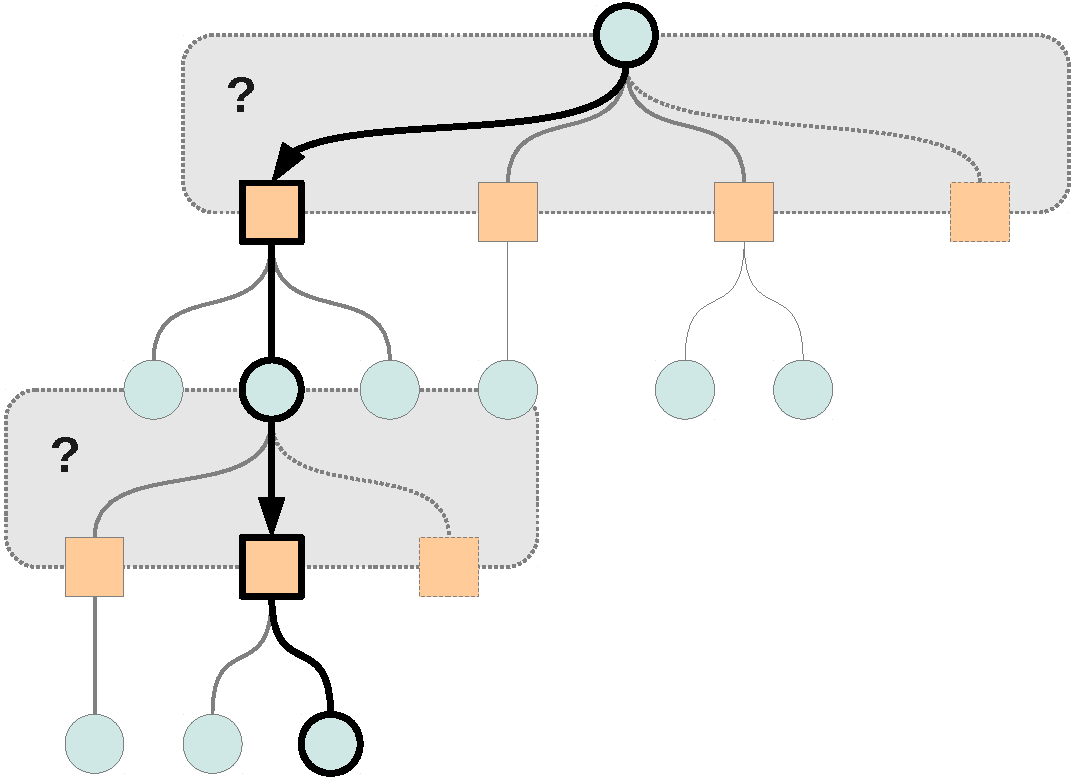
\includegraphics[width=.80\linewidth]{figs/tree3}
    \end{center}
\end{frame}


\begin{frame}{How to select the state to expand~?}
    \begin{center}
        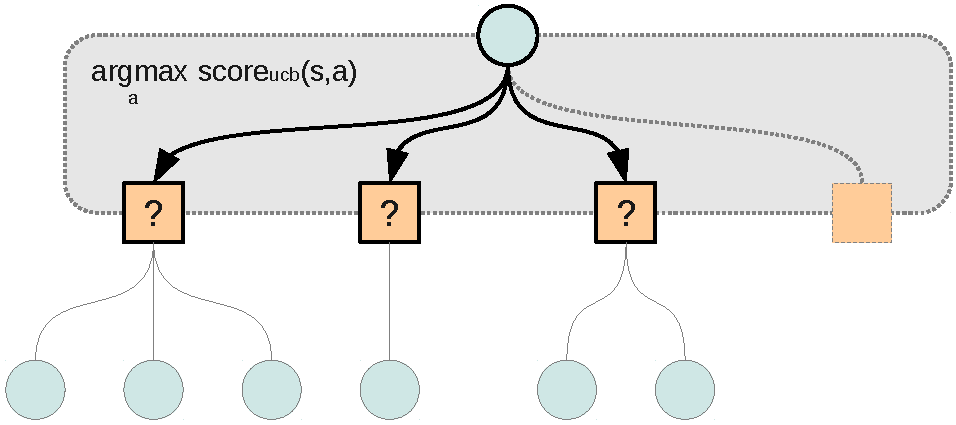
\includegraphics[width=.40\linewidth]{figs/tree4}
    \end{center}
    The {\em selection} phase is driven by \ucb{}% algorithm, knowing:
    $$
    %\scoreucb(\state, \decision) = \underbrace{\frac{1}{n_{\decision}} \sum_{0 \leq t \leq n_{\decision}}{\reward_t}}_\text{1} + K \underbrace{\sqrt{\frac{\log(N)}{n_{\decision}}}}_\text{2}
    \scoreucb(\state, \decision) = \underbrace{\hat{Q}(\state,\decision)}_\text{1} + \underbrace{\sqrt{ \frac{\log(2 + n(\state))}{2 + n(\state, \decision)} }}_\text{2}
    $$
    \only<1| handout:1> {
        \begin{enumerate}
            %\item the average reward of known actions
            \item mean reward of simulations including action $\decision$ in state $\state$
            \item the uncertainty on this estimation of the action’s value
        \end{enumerate}
    }
    \only<2| handout:2> {
        The selected action: $$\decision^\star = \arg\max_{\decision} ~ \scoreucb(\state, \decision)$$
        ~\\
    }
    ~\\
\end{frame}


\begin{frame}{How to select the state to expand~?}
    \begin{center}
        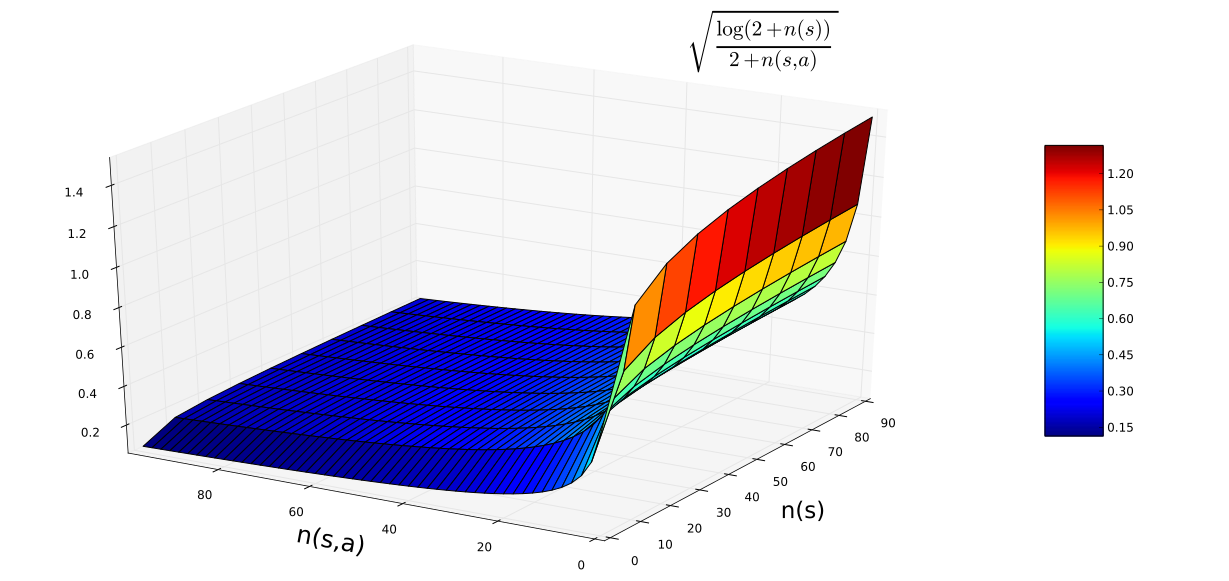
\includegraphics[width=.90\linewidth]{figs/ucb_func2}
    \end{center}
\end{frame}


\begin{frame}{When should we expand?}
    \begin{center}
        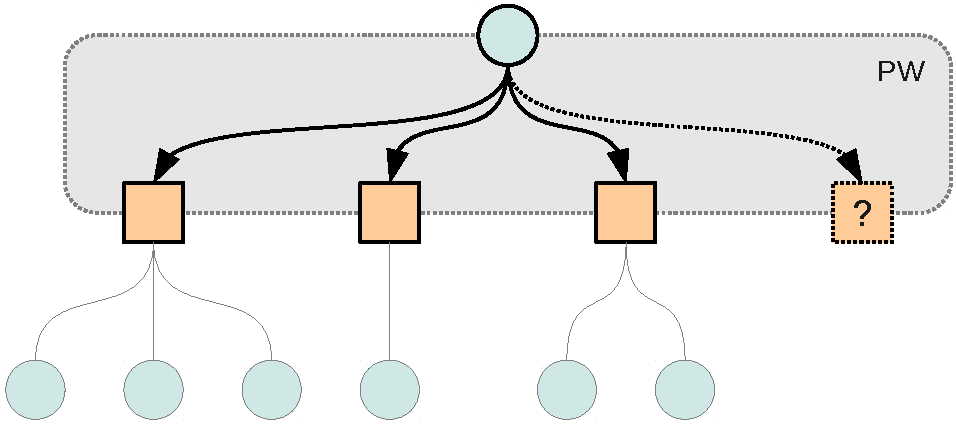
\includegraphics[width=.40\linewidth]{figs/tree5}
    \end{center}

    One standard way of tackling the exploration/exploitation dilemma
    is \pw.\\
    ~\\
    A new parameter $\alpha \in [0 ; 1]$ is introduced, to choose between exploration (add a decision to
    the tree) and exploitation (go to an existing node)
\end{frame}


\begin{frame}{How to select the state to expand~?}
    \begin{center}
        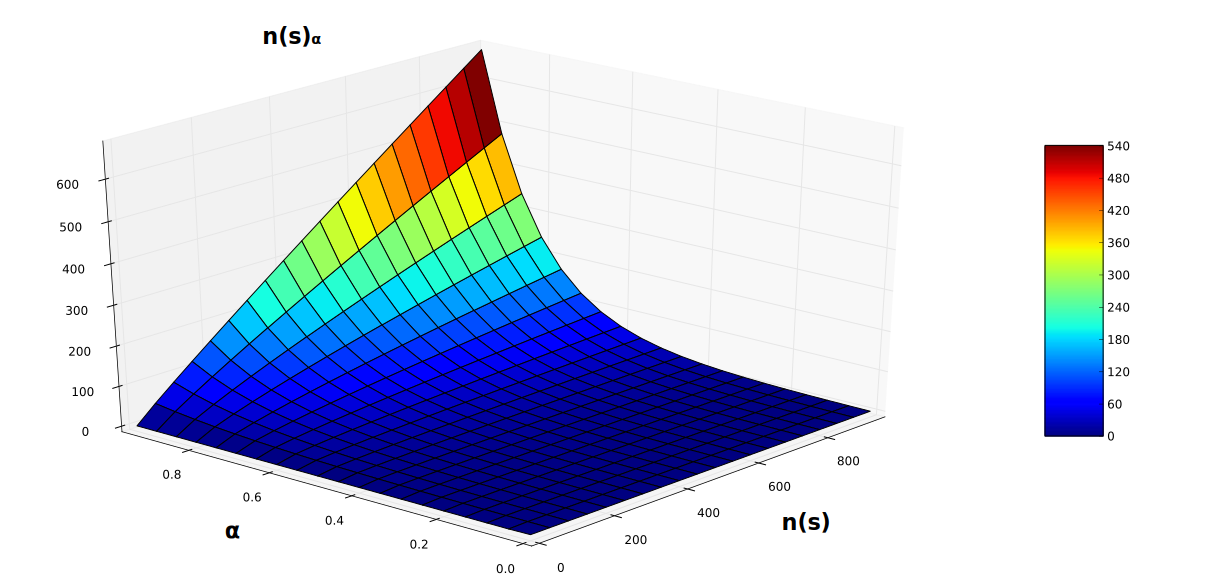
\includegraphics[width=.80\linewidth]{figs/pw_func}
    \end{center}

    \begin{itemize}
        \item $\text{if}( |\subdecisionspace{}_{\state}| < n(\state)^{\alpha} )$ then we explore a new decision
        \item else we simulate a known decision
    \end{itemize}

    With $|\subdecisionspace{}_{\state}|$ the number of legal actions in state $\state$\\
    ~\\
\end{frame}


\begin{frame}{When should we expand?}
    $\alpha = 0.2$
    \begin{center}
        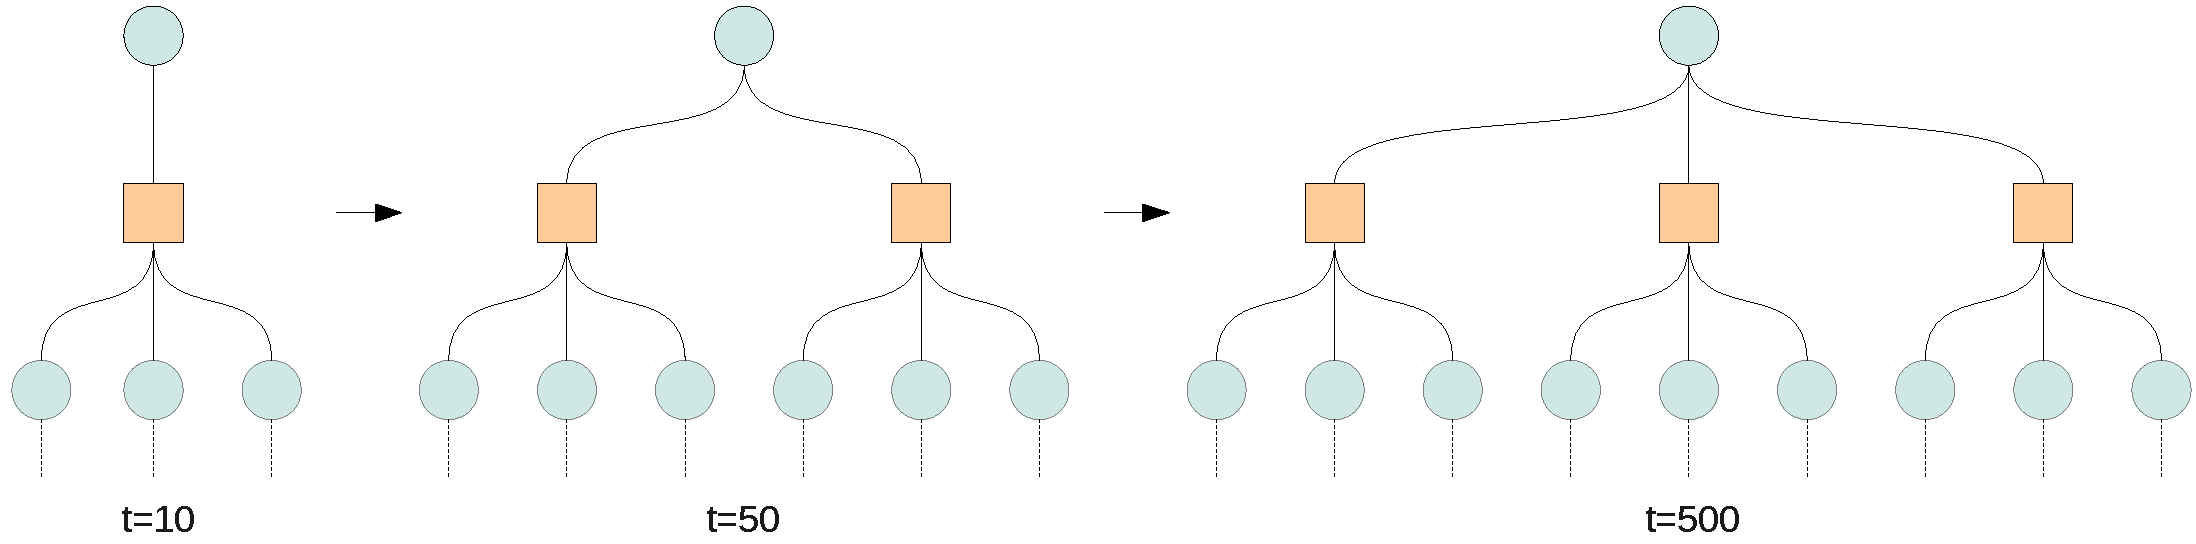
\includegraphics[width=.70\linewidth]{figs/tree6}
    \end{center}

    $\alpha = 0.8$
    \begin{center}
        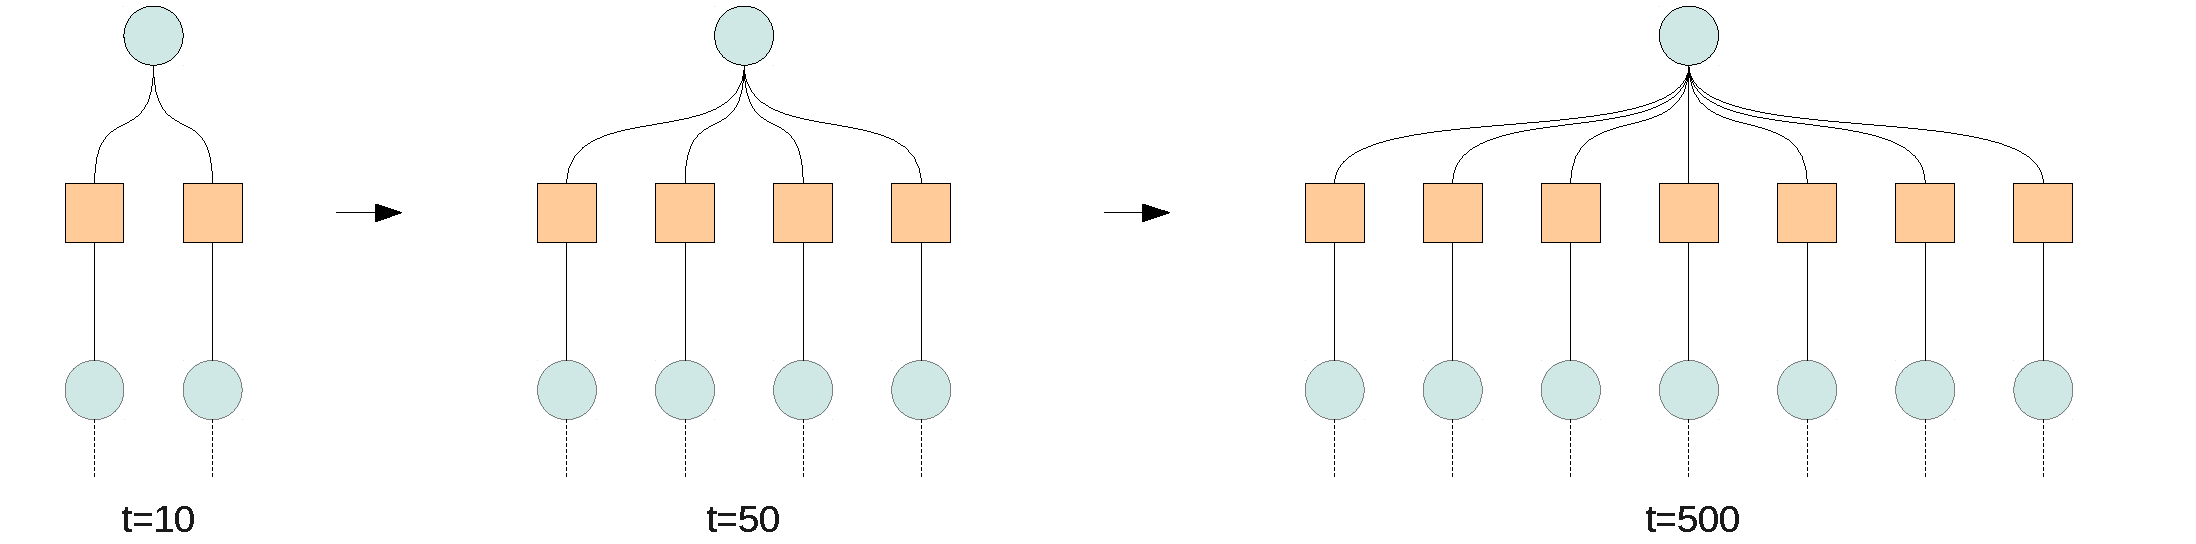
\includegraphics[width=.70\linewidth]{figs/tree7b}
    \end{center}
\end{frame}
